\chapter{DIHARD challenge setup}

This chapter discusses some specifics of the DIHARD challenge including the rules, evaluation mechanisms and datasets. Most of these details are published in \cite{ryant2019second}.

\section{Task Definition}
The goal of the challenge is to automatically split audio recordings into segments based on speaker identity. Small pauses of less than 200 ms should be merged into a single contiguous segment. During these pauses the speaker is not considered to produce any vocalization. This obviously includes speech, but also speech errors, infant babbling, breaths, coughs, lipsmacks, sneeze, laughs, humming. Basically any sound produced by the speaker by using the human vocal apparatus.

\section{Evaluation Tracks}
As a participant, there are four possible tracks to participate in. Each of these tracks have their own leaderboards. There are two input conditions - single channel audio and multichannel audio. There are also two SAD conditions - reference SAD, where manually transcribed segment boundaries are made available for use, and system SAD, where the diarization system is expected to do its own SAD on the raw audio. These conditions give rise to four possible tracks.

\section{Detail on Data Provided}

The single channel audio may be taken from a single distant microphone, or from one of the channels from a microphone array, head-mounted microphones, or a mix of these. The multichannel audio is drawn from the CHiME-5 dinner party corpus, which consists of conversational speech from dinner parties held in real homes. It is composed of several different recording sessions - each corresponding to a different party. The house had multiple arrays, so each session contains output from multiple distant microphone arrays, each containing multiple channels. Participants are required to generate one diarization output per array and are free to use any number of channels from each array. For example, if a recording session contains 4 microphone arrays, participants are expected to generate 4 RTTM files.

For the reference SAD condition, the reference segmentation has been generated by automatically merging overlapping or very close speaker turns from the human reference diarization.

\section{Scoring}
The outputs of the systems are judged by two metrics.

	\subsection{Diarization Error Rate (DER)}

		
	\subsection{Jaccard Error Rate (JER)}
	The JER metric has been newly developed for DIHARD II. It's goal is to weigh every speaker's contribution to the score equally regardless of how much speech they produce, unlike DER. This is done as follows.
	First, an optimal 1:1 mapping is determined between the reference and system speakers using the Hungarian algorithm \cite{hungarian}. Then for each pair of speakers, the Jaccard Index \cite{hamers1989similarity} is computed. The Jaccard Index measures the similarity between two sets, and is defined as their intersection size divided by union size. This is always between 0 and 1. A value of 0 implies no similarity and 1 implies maximum similarity. We can invert the meaning of 0 and 1 by subtracting it from 1, making it an error measure instead of similarity measure. We call this measure the speaker-specific JER, or $JER_{ref}$. The overall JER is then defined to be the average of $JER_{ref}$ scores for each pair.
	
	This can explained better using a Venn diagram. Suppose we have sets SYS and REF corresponding to system speaker duration and reference speaker duration respectively. The red region corresponds to the FA duration, blue region corresponds to the MISS speeech, TOTAL corresponds to the sum of all three regions.
	
	\begin{figure}[h]
		\centering
		\def\syscircle{(0,0) circle (1.5cm)}
		\def\refcircle{(0:2cm) circle (1.5cm)}
		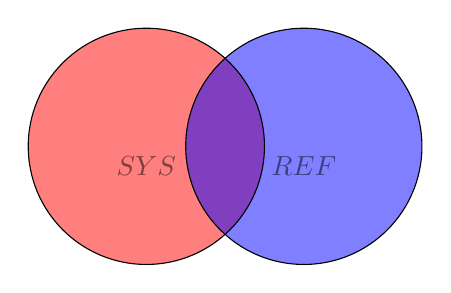
\begin{tikzpicture}
		\begin{scope}[shift={(3cm,-5cm)}, fill opacity=0.5]
		\fill[red] \syscircle;
		\fill[blue] \refcircle;
		\draw \syscircle node[below] {$SYS$};
		\draw \refcircle node [below] {$REF$};
		\end{scope}
		\end{tikzpicture}
		\caption{Jaccard Index Venn diagram}
	\end{figure}
	
	Jaccard Index is equal to the area of the purple region divided by the area of the whole colored region. The $JER_{ref}$of this would be the sum of the red and blue region, divided by the whole colored region.
	
	$$ JER_{ref} = \frac{FA + MISS}{TOTAL} $$
	
	$$ JER = \frac{1}{N}\sum_{ref}JER_{ref} $$
	
	It can be understood from this definition that the JER never exceeds 100\%.
	
\section{Datasets}
Since we work with the 2018 DIHARD datasets, we only describe their composition and not of the 2019 datasets. The development set consists of approximately 19 hours of 5-10 minute audio samples drawn from the following domains. The evaluation set consists of the samples drawn from the same domains and sources with a few exceptions. It has 21 hours of 5-10 minute long speech samples. All samples are 16 KHz single channel FLAC files.

\begin{table}[h]
	\centering
	\begin{tabular}{|c|c|}
		\hline
		Domain & Source \\
		\hline
		Child language acquisition recordings & SEEDLingS \\
		Supreme Court oral arguments & SCOTUS / OYEZ \\
		Clinical interviews & ADOS interviews \\
		Radio interviews & YouthPoint recordings \\
		Map tasks & DCIEM Map Task Corpus \\
		Sociolingustic interviews & SLX Corpus \\
		Meeting speech & RT04 datasets \\
		Audiobooks & LibriVox \\
		YouTube videos & VAST project \\
		\hline
	\end{tabular}
	\caption{Composition of DIHARD 2018 dev set.}
	\label{table-dihard-dev-composition}
\end{table}

\section{Evaluation Rules}
The DIHARD challenge is an open evaluation, and the system outputs are supposed to be generated locally and submitted to LDC for scoring. Since portions of the test data are available in following corpora that was already widely available, usage of them for training is prohibited.

	The NIST evaluations have a practice in which a forgiveness collar is applied to either sides of reference segments, to get rid of errors from inconsistent human annotations and uncertainty about when a speaker begins or ends. These collars are not scored. This does not apply for DIHARD and there are no forgiveness collars used. Overlapping speech is also evaluated - so the ideal system is expected to output overlapping segments if two speakers overlap in the source audio. A system that generates only flat segmentations (no overlap) will have higher DER because the overlapping segments could give rise to missed speech and speaker errors.

\begin{itemize}
	\item DCIEM Map Task Corpus (LDC96S38)
	\item MIXER6 Speech (LDC2013S03)
	\item Digital Archive of Southern Speech (LDC2012S03 and LDC2016S05)
	\item NIST SRE10 evaluation data
	\item NIST SRE12 evaluation data
	\item DIHARD I evaluation sets
	\item the SEEDLingS subset of HomeBank
\end{itemize}

Human investigation of the evaluation data is not allowed. Participants are allowed to automatically derive information using the development and evaluation sets.
